\section{Hardware Overview}

\subsection{Sensors}
\subsubsection{Ultrasonics}
Active ultrasonic sensors generate high-frequency sound waves and evaluate the echo which is received back by the sensor, measuring the time interval between sending the signal and receiving the echo to determine the distance to an object.
\begin{figure}[!htb]
\begin{center}
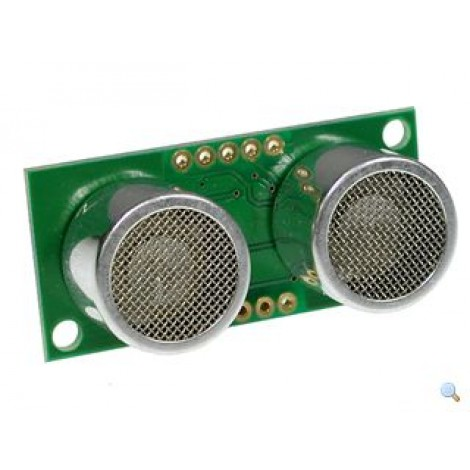
\includegraphics[width=3cm]{ultrasonics.jpg}
\end{center}
\caption{Ultrasonics}
\label{fig:Ultrasonics}
\end{figure}

\subsubsection{Motor Encoders}
A rotary encoder, also called a shaft encoder, is an electro-mechanical device that converts the angular position or motion of a shaft or axle to an analog or digital code. 

\subsubsection{Kinect}
A powerful camera and microphone. The camera can provide a colour stream, a depth stream and an infra-red stream. The array microphone allows sound localisation. 
\begin{figure}[!htb]
\begin{center}
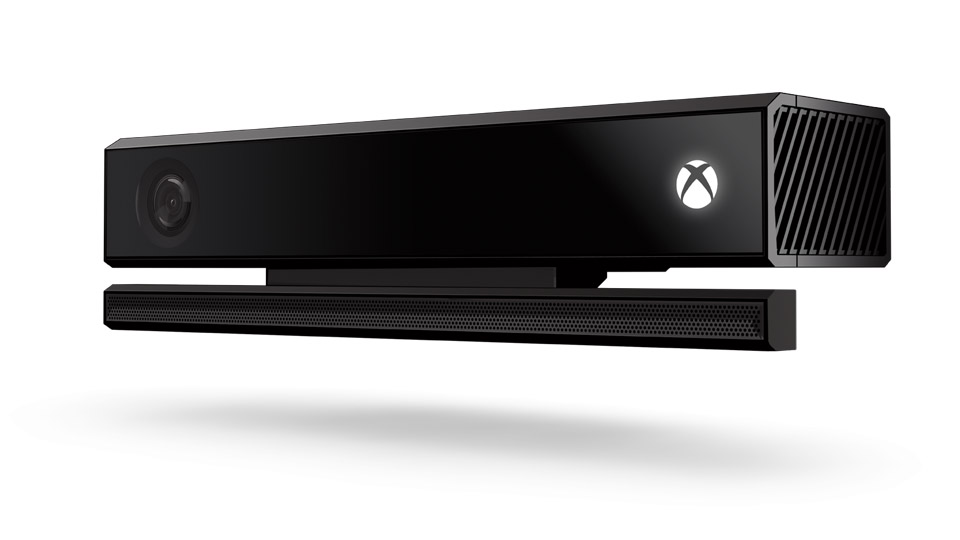
\includegraphics[width=3cm]{kinect.jpg}
\end{center}
\caption{kinect}
\label{fig:kinect}
\end{figure}

\subsection{Compute Power}
\subsubsection{Raspberry Pi}
The Raspberry Pi is a low cost, credit-card sized computer that plugs into a computer monitor, and uses a standard keyboard and mouse. It has 20 GPIO pins; these allow it to be connected to an I2C network. 
\begin{figure}[!htb]
\begin{center}
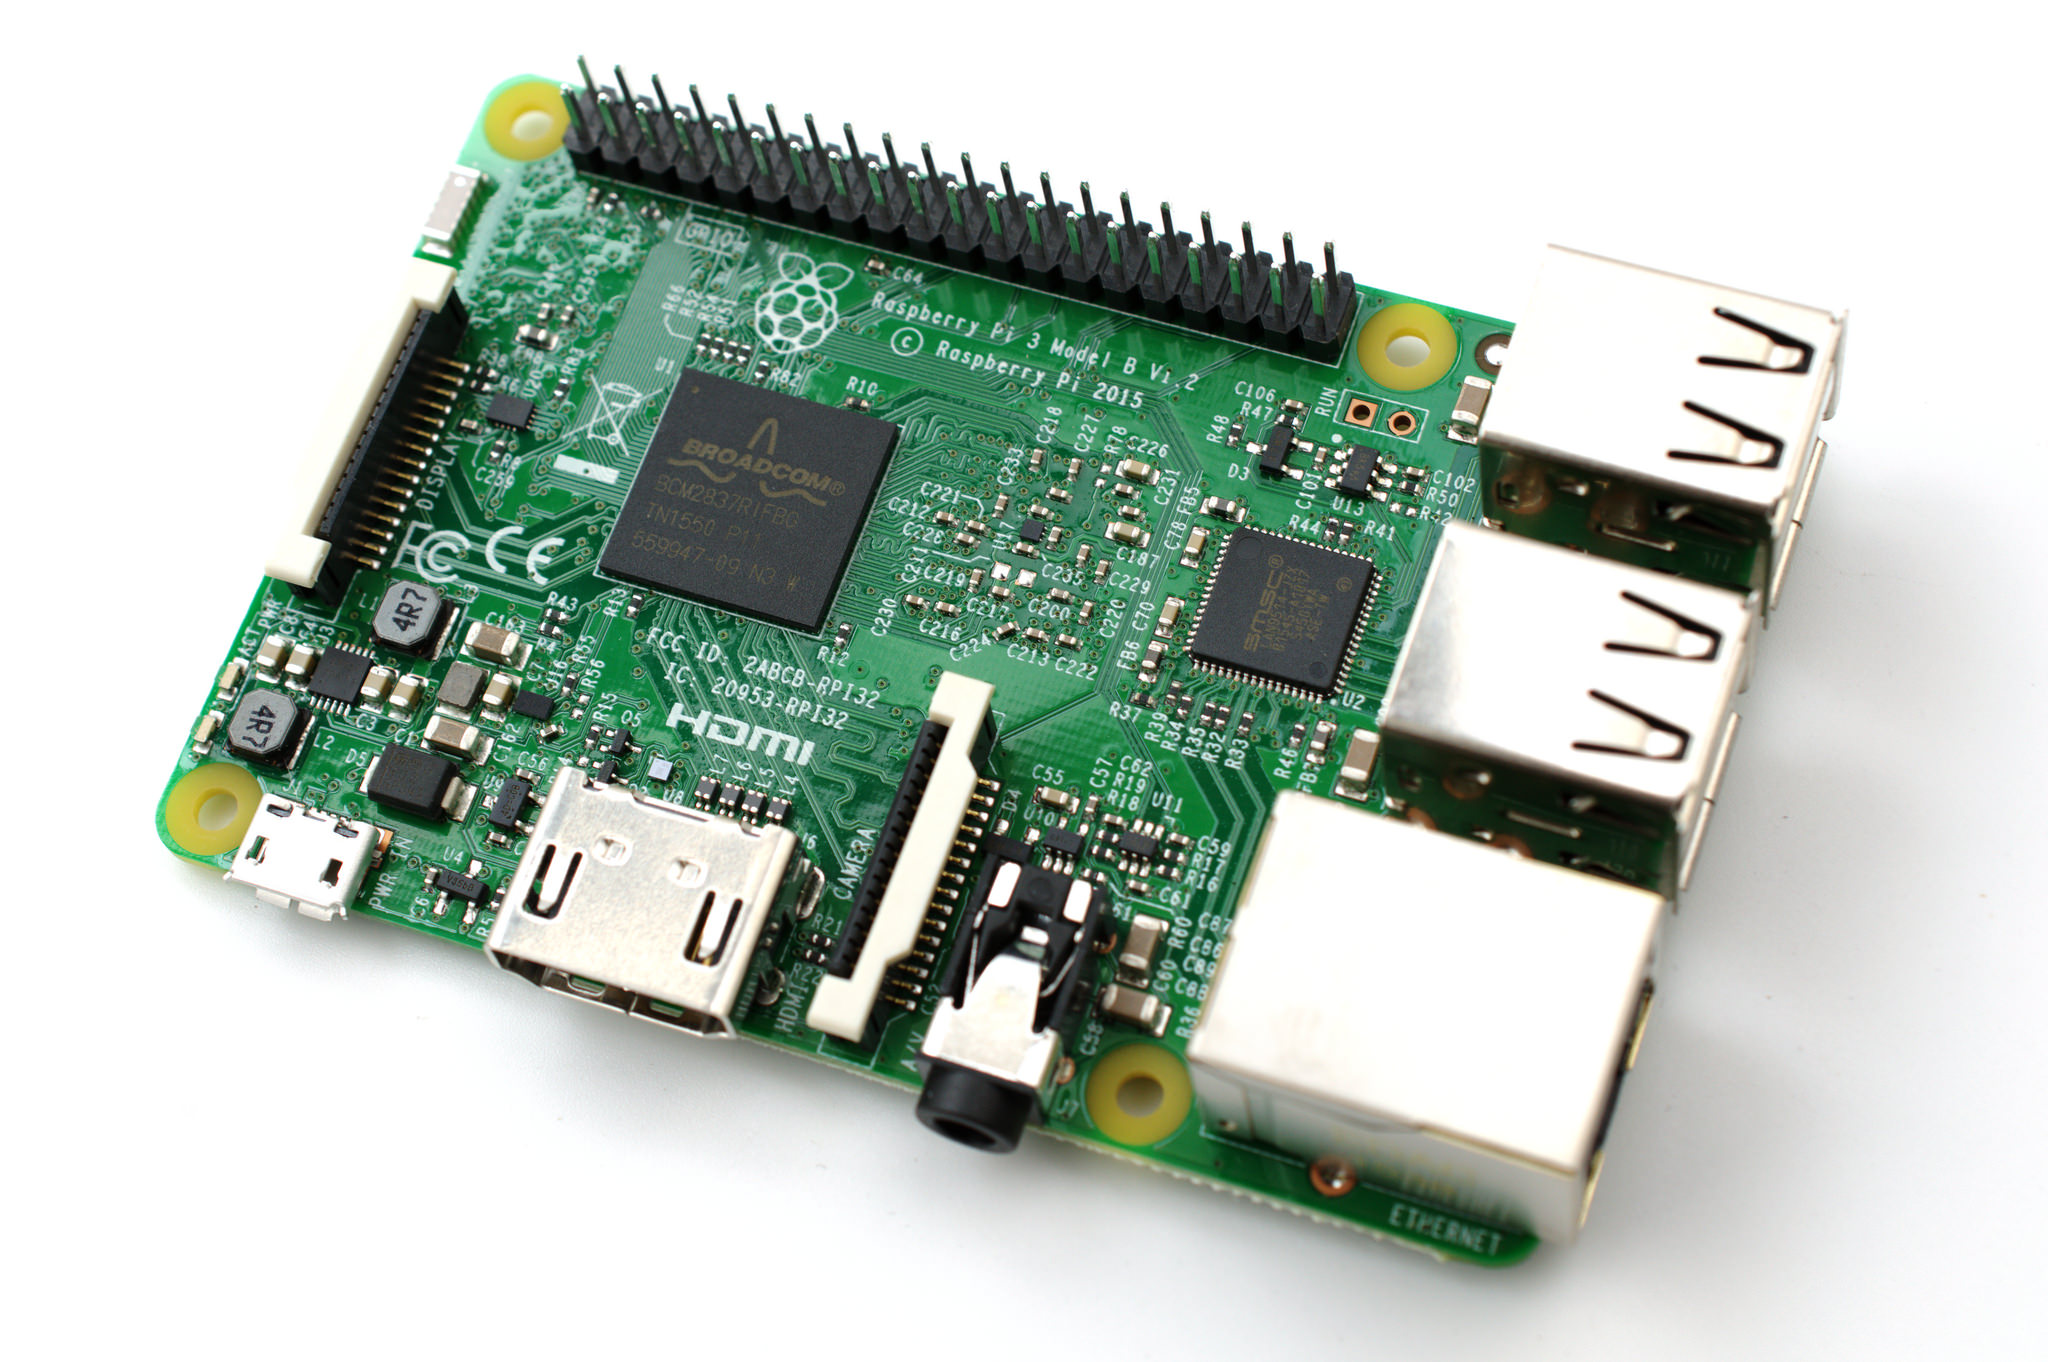
\includegraphics[width=3cm]{raspberrypi.jpg}
\end{center}
\caption{raspberrypi}
\label{fig:raspberrypi}
\end{figure}

\subsubsection{Kinect PC}
The Kinect PC is a motherboard with an attached SSD. It requires a USB 3.0 connection to interface with the Kinect. 

\subsubsection{SSD}
A storage device containing non-volatile flash memory, used in place of a hard disk because of its much greater speed. This is used in conjunction with a PC.

\subsubsection{mbed}
ARM® mbed™ IoT Device Platform, simply, is for writing software that controls hardware that can connect to the cloud - it is an easy way of creating embedded connected solutions.
\begin{figure}[!htb]
\begin{center}
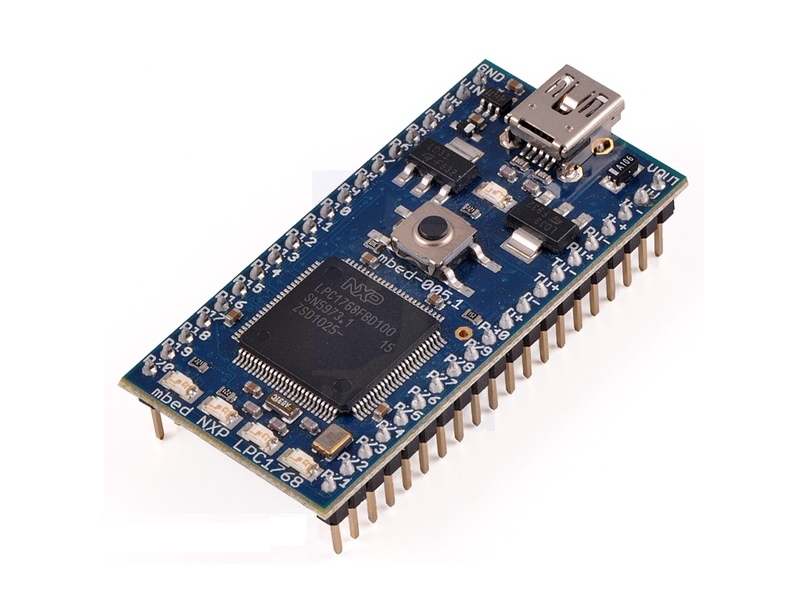
\includegraphics[width=3cm]{mbed.jpg}
\end{center}
\caption{mbed}
\label{fig:mbed}
\end{figure}

\subsubsection{Arduino}
A pre-assembled Arduino board includes a microcontroller, which is programmed using Arduino programming language and the Arduino development environment. In essence, this platform provides a way to build and program electronic components. Arduino programming language is a simplified from of C/C++ programming language based on what Arduino calls "sketches," which use basic programming structures, variables and functions. These are then converted into a C++ program. 

Two versions of Arduino are on-board Tiberius. One is the nano and the other is a mega.

\begin{figure}[!htb]
\begin{center}
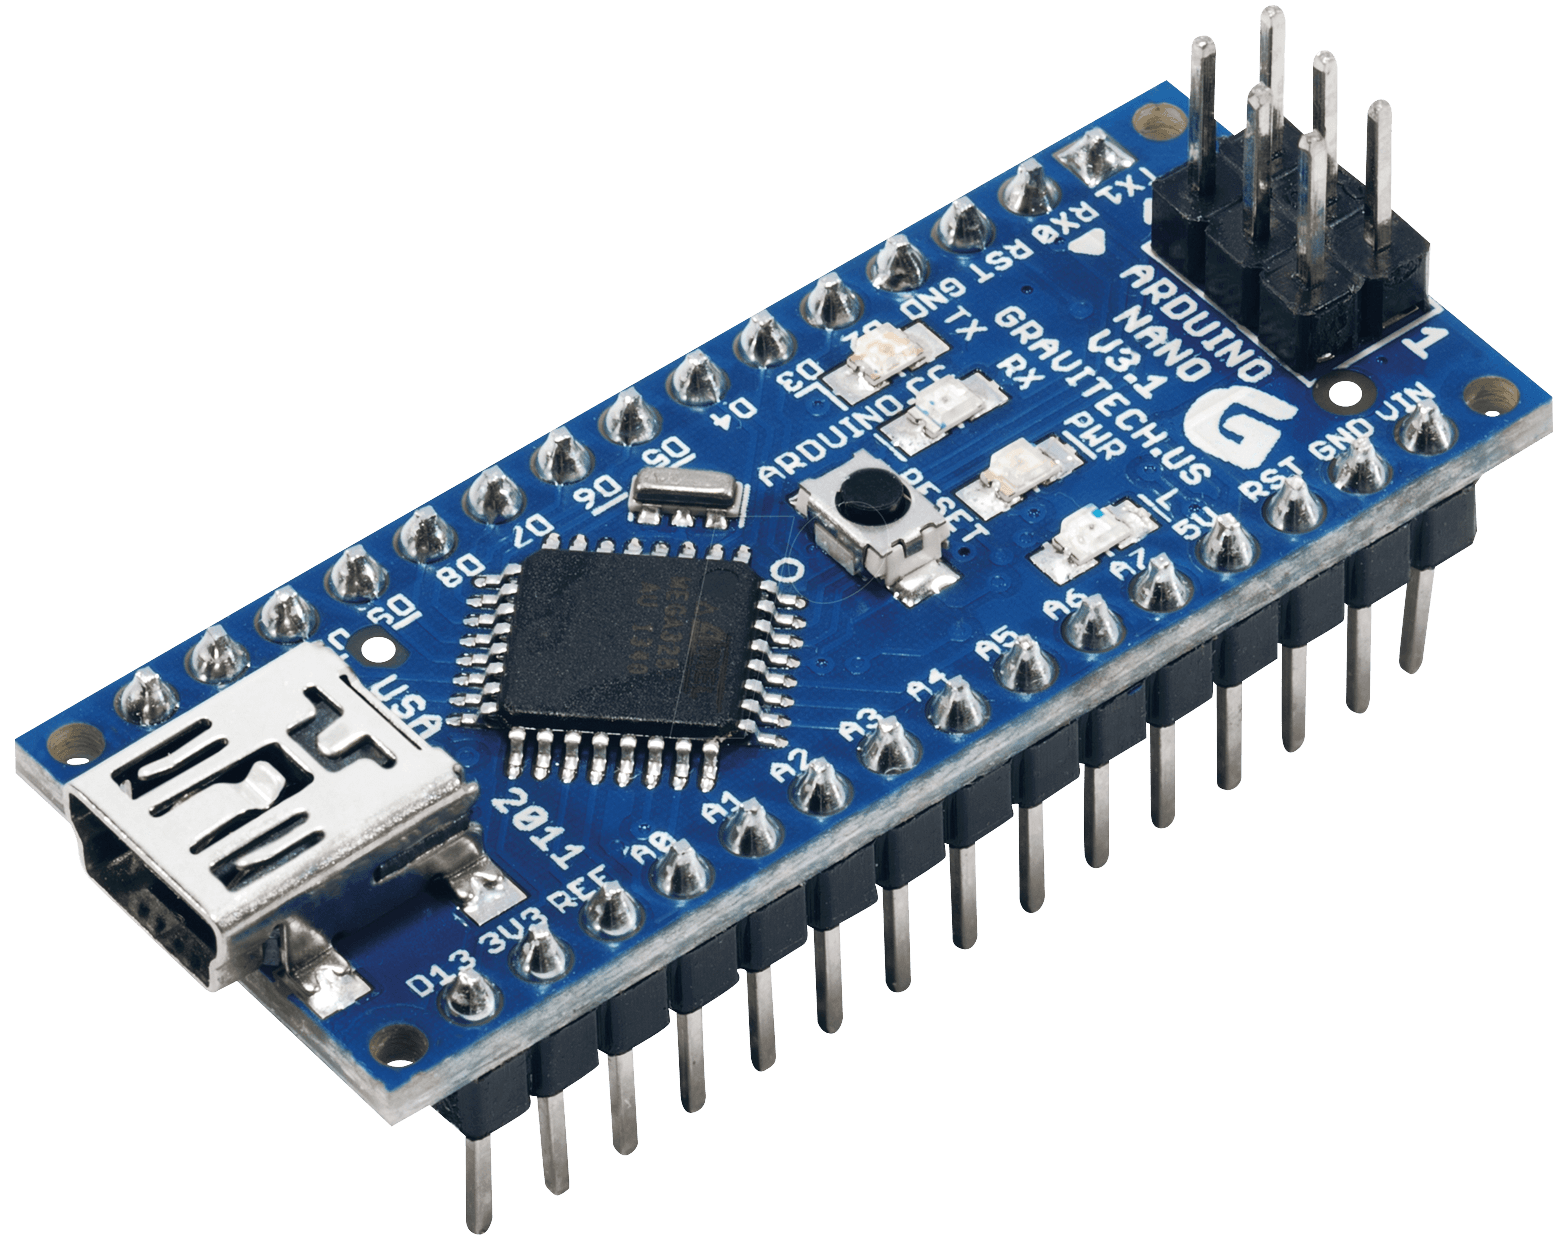
\includegraphics[width=3cm]{arduinonano.png}
\end{center}
\caption{arduino nano}
\label{fig:arduinoNano}
\end{figure}

\begin{figure}[!htb]
\begin{center}
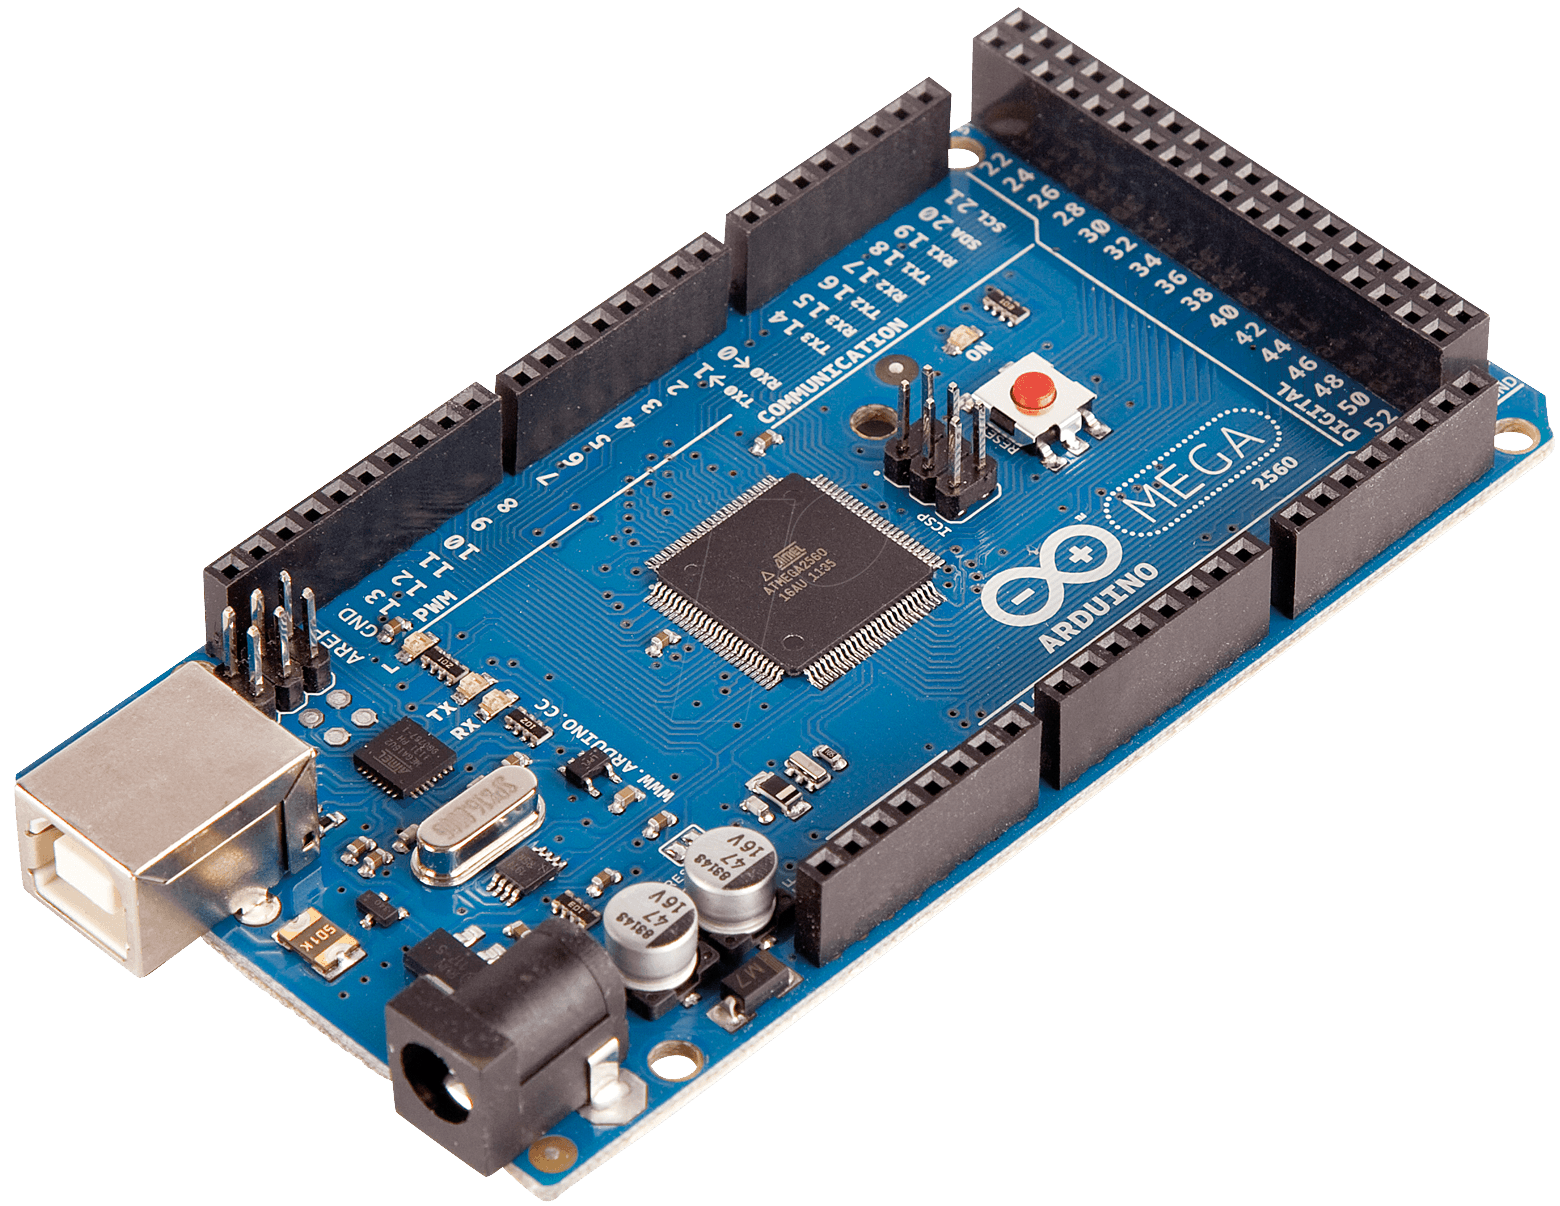
\includegraphics[width=3cm]{ARDUINO_MEGA.png}
\end{center}
\caption{Arduino mega}
\label{fig:ArduinoMega}
\end{figure}

\subsubsection{RAMPS board}
Tiberius implements a 1.4 ramps board.
\begin{figure}[!htb]
\begin{center}
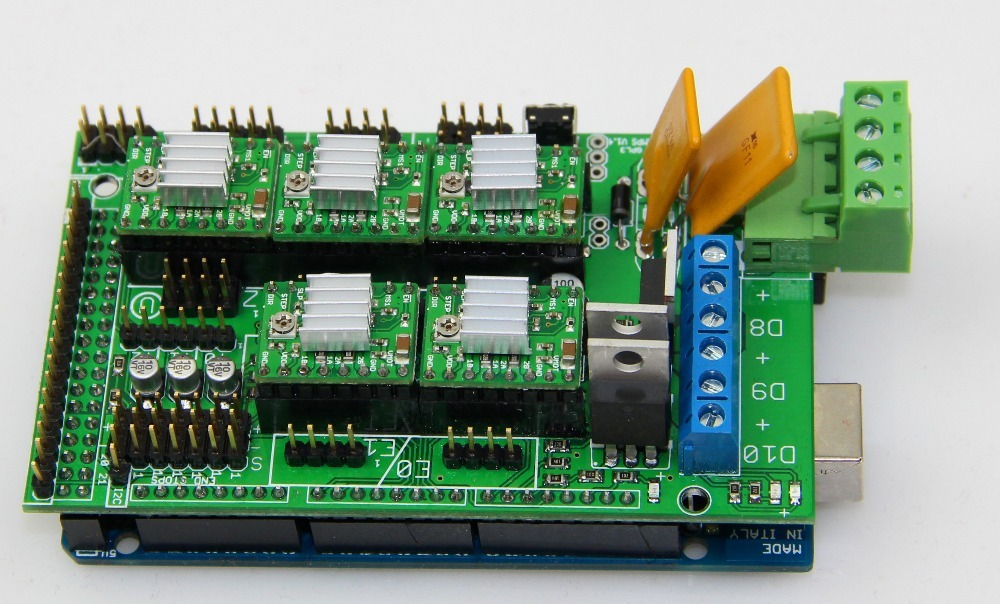
\includegraphics[width=3cm]{ramps.jpg}
\end{center}
\caption{ramps}
\label{fig:ramps}
\end{figure}

\subsubsection{MD03 Motor drivers}
% http://www.robot-electronics.co.uk/htm/md03tech.htm 
The MD03 is a medium power motor driver, designed to supply power beyond that of any of the low power single chip H-Bridges that exist. Main features are ease of use and flexibility. The motor's power is controlled by Pulse Width Modulation (PWM) of the H-Bridge at a frequency of 15khz ( 7.5khz before version 12). 
\begin{figure}[!htb]
\begin{center}
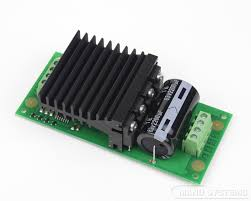
\includegraphics[width=3cm]{md03.jpg}
\end{center}
\caption{md03}
\label{fig:md03}
\end{figure}



\subsection{Actuators}
\subsubsection{Robot Arm}
The robotic arm has 3 joints and a free hanging gripper. It has a lifting capacity of 2Kg. It is controlled by an Arduino and can be either controlled using joint positions or Cartesian coordinates.
\subsubsection{Motors}
% http://www.mfacomodrills.com/gearboxes/986d_series.htm
% this link has the motor info on it.
Designed for heavy-duty industrial and model applications this robust unit boasts a powerful high quality motor with scintered bronze bearings. The metal gearbox incorporates ballrace bearings, enabling the high torque transfer from the motor to be
transmitted through the gearbox. The extended rear motor shaft can facilitate encoder installation \cite{Dun_dcmotor}.
\begin{figure}[!htb]
\begin{center}
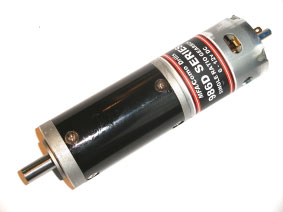
\includegraphics[width=3cm]{motor.jpg}
\end{center}
\caption{motor}
\label{fig:motor}
\end{figure}


